\documentclass[border=10pt]{standalone}
\usepackage{amsmath}
\usepackage{pgfplots}
\usepgfplotslibrary{fillbetween}
\pgfplotsset{compat=1.16}
\begin{document}
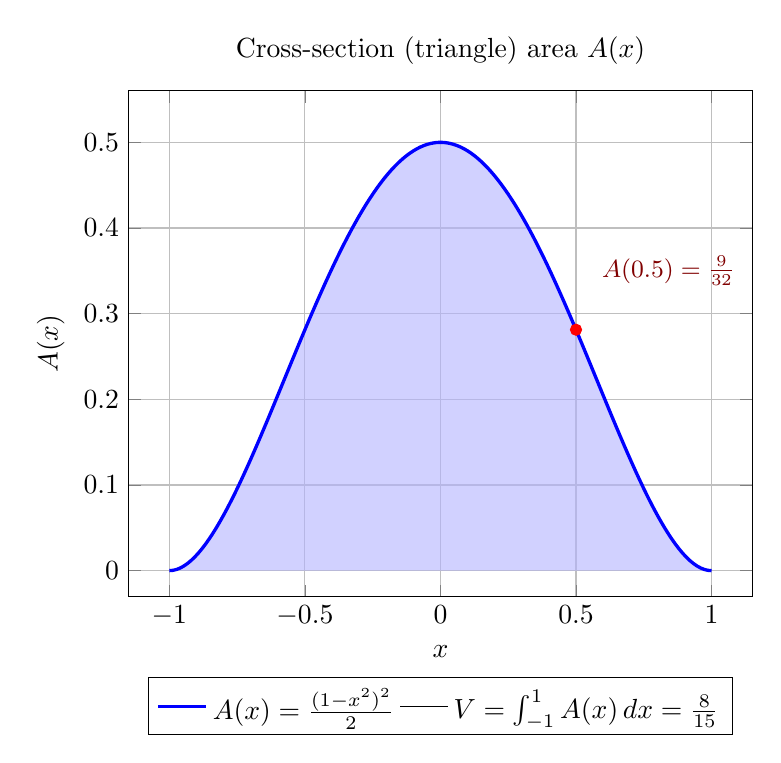
\begin{tikzpicture}
\begin{axis}[
    width=9.5cm, height=8cm,
    xlabel={$x$}, ylabel={$A(x)$},
    xmin=-1.15, xmax=1.15, ymin=-0.03, ymax=0.56,
    xtick={-1,-0.5,0,0.5,1}, ytick={0,0.1,...,0.5},
    grid=major, title={Cross-section (triangle) area $A(x)$},
    legend style={at={(0.5,-0.16)}, anchor=north, legend columns=2},
    legend cell align=left,
]
\addplot[name path=Acurve, blue, very thick, domain=-1:1, samples=150] {(1-x^2)^2/2};
\addlegendentry{$A(x)=\frac{(1-x^2)^2}{2}$}
\addplot[name path=Aaxis, draw=none, domain=-1:1, samples=2] {0};
\addplot[blue!30, opacity=0.6] fill between[of=Acurve and Aaxis];
\addlegendentry{$V=\int_{-1}^{1}A(x)\,dx=\frac{8}{15}$}
\addplot[only marks, mark=*, red] coordinates {(0.5,0.28125)};
\node[anchor=west, text=red!50!black] at (axis cs:0.56,0.35) {\small $A(0.5)=\frac{9}{32}$};
\end{axis}
\end{tikzpicture}
\end{document}
